\documentclass{article}
\usepackage[T1]{fontenc}
\usepackage{lmodern}
\usepackage{graphicx}
\usepackage{amsmath,amssymb}
\usepackage[a4paper,margin=2cm]{geometry}
\usepackage[absolute,overlay]{textpos}
\setlength{\TPHorizModule}{1mm}
\setlength{\TPVertModule}{1mm}
\usepackage[indonesian]{babel}
\usepackage{hyperref}
\setlength{\emergencystretch}{2em}
% unit: Halaman 51

\begin{document}

% === Halaman 51 (llm) ===

\vspace{98.90mm}

\section*{Prinsip \textit{Confusion} dan \textit{Diffusion}}

\begin{itemize}
    \item Claude Shannon dalam makalah klasiknya tahun 1949, \textit{Communication theory of secrecy systems}, memperkenalkan prinsip \textit{confusion} dan \textit{diffusion} untuk membuat serangan berbasis statistik terhadap \textit{cipher} menjadi lebih sulit dilakukan.
    \vspace{10mm}
    \item Dua prinsip tersebut, \textit{confusion} dan \textit{diffusion}, menjadi panduan dalam merancang algoritma kriptografi, baik \textit{stream cipher} maupun \textit{block cipher}.
\end{itemize}

% deskripsi: Foto potret Claude Shannon
% bbox normalisasi: [0.7930, 0.1300, 0.9260, 0.4630]
\begin{textblock*}{27.93mm}(166.53mm,38.61mm)
\noindent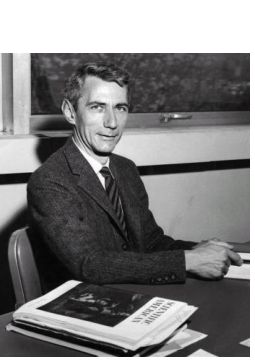
\includegraphics[width=27.93mm,height=98.90mm]{../../images/llm/page_051_img_01.png}%
\end{textblock*}

\end{document}
